\documentclass[10pt,a4paper,twocolumn]{article}

\usepackage[top=2.2cm,bottom=2.2cm,left=1.8cm,right=1.8cm,columnsep=0.7cm]{geometry}
\usepackage[T1]{fontenc}
\usepackage[utf8]{inputenc}
\usepackage{libertine}
\usepackage[varqu,varl]{inconsolata}
\usepackage{microtype}
\usepackage{graphicx}
\usepackage{booktabs}
\usepackage{tabularx}
\usepackage{array}
\usepackage{enumitem}
\usepackage{xcolor}
\usepackage{caption}
\usepackage{float}
\usepackage{fancyhdr}
\usepackage{titlesec}
\usepackage{tikz}
\usepackage{pgfplots}
\usepackage[most]{tcolorbox}
\usepackage{xurl}
\usepackage{hyperref}

\usetikzlibrary{positioning,arrows.meta}
\pgfplotsset{compat=1.16}

% ---------------------------------------------------------------- colours
\definecolor{maroon}{HTML}{7A1F2B}
\definecolor{maroonlight}{HTML}{F6ECEC}
\definecolor{ink}{HTML}{2B2B2B}
\definecolor{muted}{HTML}{6B6B6B}
\definecolor{cBlue}{HTML}{2A78D6}
\definecolor{cOrange}{HTML}{EB6834}
\definecolor{cGreen}{HTML}{1BAF7A}
\definecolor{cGrey}{HTML}{8A8983}

\hypersetup{colorlinks=true, linkcolor=maroon, urlcolor=maroon, citecolor=maroon,
  pdftitle={The Mountain Year and Its Owners: Stage 2 report},
  pdfauthor={Vishak Kashyap K, Vedant Kulkarni, Himangi Sahoo}}

% ---------------------------------------------------------------- layout
\setlist{itemsep=2pt,topsep=4pt,parsep=0pt}
\setlength{\parindent}{0pt}
\setlength{\parskip}{4pt}
\renewcommand{\topfraction}{0.9}\renewcommand{\bottomfraction}{0.8}\renewcommand{\textfraction}{0.07}\renewcommand{\floatpagefraction}{0.75}\renewcommand{\dbltopfraction}{0.9}\renewcommand{\dblfloatpagefraction}{0.75}
\renewcommand{\arraystretch}{1.18}
\emergencystretch=3em
\captionsetup{font=small,labelfont={bf,color=maroon},labelsep=period}
\graphicspath{{analysis/}}

\titleformat{\section}{\Large\sffamily\bfseries\color{maroon}}{\thesection}{0.7em}{}[{\color{maroon!35}\titlerule}]
\titleformat{\subsection}{\large\sffamily\bfseries\color{maroon!85!black}}{\thesubsection}{0.6em}{}
\titlespacing*{\section}{0pt}{16pt}{8pt}
\titlespacing*{\subsection}{0pt}{12pt}{4pt}

\pagestyle{fancy}
\fancyhf{}
\fancyhead[L]{\small\sffamily\color{muted}The Mountain Year and Its Owners}
\fancyhead[R]{\small\sffamily\color{muted}Stage 2: the sources and the computational analysis}
\fancyfoot[C]{\small\sffamily\color{maroon}\thepage}
\renewcommand{\headrule}{{\color{maroon!30}\hrule height 0.4pt}}

\newcommand{\file}[1]{\texttt{\detokenize{#1}}}
\newcommand{\pg}[2]{(#1, p.~#2)}
\newcommand{\entry}[1]{{\small\sffamily\color{muted}[#1]}}

\newtcolorbox{finding}{enhanced, colback=maroonlight, colframe=maroonlight, boxrule=0pt, arc=2pt,
  borderline west={3pt}{0pt}{maroon}, left=10pt, right=10pt, top=6pt, bottom=6pt, before skip=8pt, after skip=8pt}

\begin{document}

% ================================================================ title page
\begin{titlepage}
\centering
\vspace*{1.5cm}
{\large Introduction to History (HS3.201)\par}
{\large International Institute of Information Technology, Hyderabad\par}
\vspace{2.5cm}
{\color{maroon}\rule{0.6\textwidth}{0.6pt}\par}
\vspace{0.6cm}
{\Huge\bfseries\color{maroon}The Mountain Year and Its Owners\par}
\vspace{0.4cm}
{\Large\itshape\color{maroon!80!black}Seasonal herding in the Himachal hills, 1881--1961\par}
\vspace{0.6cm}
{\color{maroon}\rule{0.6\textwidth}{0.6pt}\par}
\vspace{1cm}
{\large Stage 2 Report: Working with the Sources and the Computational Analysis\par}
\vspace{2cm}
{\large Vishak Kashyap K\par}
\vspace{0.15cm}
{\large Vedant Kulkarni\par}
\vspace{0.15cm}
{\large Himangi Sahoo\par}
\vspace{1.2cm}
{\large\color{muted}14 October 2026\par}
\vfill
{\small\color{muted}Code, data and outputs:\par}
\vspace{2pt}
{\small\url{https://github.com/gamemaker1/history/tree/analysis}\par}
\vspace{1cm}
\end{titlepage}
\onecolumn

% ================================================================ summary + contents
\section*{Summary}
\addcontentsline{toc}{section}{Summary}

This report is about the middle stage of our project: what we did with the sources, and what our computations show so far. Our sources are the 1961 Census village surveys of Himachal Pradesh, read alongside the 1881 and 1931 Punjab censuses and H.~A.~Rose's \emph{Glossary of the Tribes and Castes}. Together they come to about 580~MB of scans and more than four million words of OCR text, far too much to read line by line.

So we worked in two moves. First we read the whole corpus at a distance. We counted herding words in every volume, scored every page, and picked out the 510 pages that matter most. Then we read those pages closely, with help, and turned what they say into an \emph{evidence graph}: 1,964 short statements such as ``the Brahmans of Brahmaur own 2,027 sheep and goats'', each tied to the exact words and the page it comes from. A script refuses any statement whose quotation it cannot find on the cited page. On top of this graph we built a seasonal calendar, ownership tables by caste, a test of altitude against flock size, a series of the flocks that paid grazing fees, a chart of who took a share of whose product, a route map, and a check of which sources copy which.

The results so far point one way. The herding year itself hardly changed between 1881 and 1961: the same months and the same routes appear in sources that do not copy each other, and big flocks are found only high up in the Ravi, Sutlej and Chenab valleys. The flocks stayed with the landholding castes, who owned about 89\% of the animals in the survey tables. What changed was who took a cut. In the princely period it was the raja and the man who bought from him the right to collect grazing fees. After 1948 it was the Forest Department, whose permits soon became something shepherds bought and sold, and all along it was the moneylender and the shopkeeper. Geography set the shape of the mountain year; property and the state decided who gained from it.

\vspace{4pt}
{\hypersetup{linkcolor=ink}\setcounter{tocdepth}{1}\tableofcontents}

% ================================================================ 1
\twocolumn
\section{What this stage asked of us}

The brief for this stage asks us to show how we worked with the sources and what our computational analysis is: to examine and organise the information in the sources, to use suitable methods to explore it, to find patterns and relationships, and to compare across sources where that helps. Our research question, from Stage~1, is:

\begin{quote}\itshape How did the seasonal movement of flocks between high summer pastures and low winter grazing shape life in the Himachal hills between 1881 and 1961, and who controlled and profited from it? As rule over the hills, control of the pastures, roads and trade changed, did the herding cycle persist as an adaptation to mountain and season, or did the ownership of flocks, pastures and shepherds' labour reshape it?\end{quote}

This report is organised around the tasks of the brief. Section~\ref{sec:sources} describes the sources and how we put them in order. Section~\ref{sec:method} explains the method and why we chose it. Section~\ref{sec:findings} goes through what each analysis found. Section~\ref{sec:compare} compares the sources with each other, and Section~\ref{sec:checks} records how we checked the work, what we got wrong on the way, and where AI tools did part of it. Section~\ref{sec:next} says what is still to be done.

We read the sources in two ways, as the course asked. The \textbf{Annales reading} follows Braudel's three speeds of time: the slow time of mountain, snow and route; the medium time of economic and political arrangements; and the quick time of events such as the 1948 merger. It also borrows Bloch's habit of comparing places that share conditions but differ in one respect. The \textbf{Marxist reading} asks who owned the flocks and the pastures, who did the herding, and how the owners took a share of the product, whether as rent, fees, revenue or interest. We split the question into three parts:

\begin{description}[leftmargin=1.5em,style=nextline,font=\sffamily\bfseries\color{maroon}]
\item[SQ1. The cycle] What were the herding calendar and routes in each village, and do the 1961 surveys agree with the colonial sources of 1881, 1911 and 1931?
\item[SQ2. Ownership and labour] Who owned the flocks, who herded them, and who owned the pastures and collected dues before and after 1948?
\item[SQ3. Change by 1961] What happened to the flocks under the permit system, and what do the surveys tie to change: permits, roads, road wages, the closed Tibet border, orchards?
\end{description}

A note on page numbers: throughout, we give the PDF page (the counter a PDF viewer shows), not the number printed on the scan, and we cite in the form \pg{Brahmaur}{54}. Anyone with the repository can find the page of a quotation with one command, for example \file{python3 scripts/pageref.py find "grazing rights belonged to the rajah"}, which answers Newell, p.~18. Everything here can be rerun from our repository, \url{https://github.com/gamemaker1/history/tree/analysis}, which holds the sources, every script, the data and a log of each step (\file{computational-analysis.md}); entry numbers in square brackets, such as \entry{A10}, point to that log.

% ================================================================ 2
\section{The sources and how we organised them}\label{sec:sources}

\subsection{Four layers of evidence}

Our sources fall into four layers. Three are colonial and one belongs to the 1961 Census, and the 1961 layer is by far the largest.

\begin{table*}[!t]
\centering\small
\begin{tabularx}{\textwidth}{@{}>{\bfseries\color{maroon}}l>{\raggedright\arraybackslash}X>{\raggedright\arraybackslash}X@{}}
\toprule
\textcolor{ink}{Layer} & \textbf{What it is} & \textbf{What we use it for}\\
\midrule
1881 & Denzil Ibbetson, \emph{Report on the Census of the Panjab, 1881}, Results volume and five other parts & Barnes's description of the Gaddis: flocks in Kangra in winter and Chamba in summer, and fined by two rulers \pg{1881}{275}\\
1911 & H.~A.~Rose, \emph{A Glossary of the Tribes and Castes of the Punjab and North-West Frontier Province}, 3 volumes (1911--1919) & The Gaddi year by month \pg{Rose}{297}; the hill Gujjars\\
1931 & \emph{Census of India 1931}, Vol.~XVII, Punjab, Part~I (Report) and Part~II (Tables) & The winter movement of hill people and flocks \pg{1931}{142}\\
1961 & 24 village survey monographs of Himachal Pradesh, and four 1961 reports: William Newell's study of the Gaddis, the Weaving Craft Survey, and the Mahasu and Simla district handbooks & Flocks by caste, pastures, dues, permits, labour, debt and trade; Newell for the raja's grazing rights and the fee-paying flocks\\
\bottomrule
\end{tabularx}
\caption{The four source layers.}
\end{table*}

The village volumes alone hold about 1.15 million words of OCR text, and about 1.6 million with the four reports. There are 24 village volumes, not 25, because the Kupha volume covers four villages of Pangi (Kupha, Parmas, Thamoh and Malet) and the 25th monograph in the archive, Mahsa Tibba, is a village in Ambala, outside the hills. We left it out.

\subsection{Making the corpus trustworthy}

Before counting anything, we had to be sure that a page in our text files is the same page in the scan. Otherwise every citation would be off. We did four things \entry{A0, A1}.

First, we unpacked the archives and removed duplicates by checksum. The two zip files hold 49 PDFs, but only 40 are different: 34 from 1961 and 6 from 1881. Second, we checked each text file against its PDF. Every text file marks the end of a page with a form feed, so we counted the form feeds and compared them with the number of pages in the PDF. All 44 files match exactly, so a page found through the text is the right page in the scan. Third, we put the shared code (file paths, rejoining words broken by hyphens, cleaning text) into one module, so that every later script reads the sources the same way. Fourth, we wrote two small tools: one finds the page of any quotation, and the other turns a page into an image. The second matters because OCR scrambles tables, and the livestock tables are some of our most important evidence.

A quick test showed the chain works. Rendering Brahmaur, p.~54 gives the table of flocks by caste exactly as we had copied it in Stage~1: Brahmans 34 households, 20 of them with flocks, 2,027 animals; Rajputs 49, 20 and 2,364; Sipis 15, 8 and 93; in all 99 households, 48 with flocks, 4,484 animals.

\subsection{What the corpus cannot do}

The OCR is uneven, and tables suffer most. Some passages we cite are correct on the page but garbled in the text: Newell's ``wool in lieu of revenue'' (p.~14) comes out of the OCR as a jumble of symbols, so a word search cannot find it. For that reason we read tables from page images and mark such figures as image-read. The colonial volumes also cover the whole of Punjab, plains as well as hills, so their word counts are diluted, and they can be compared with each other but not directly with a single village.

% ================================================================ 3
\section{The method: from distant reading to an evidence graph}\label{sec:method}

\subsection{The pipeline}

Our method moves in steps from the whole corpus to a small set of checked statements, and from those to the analyses (Figure~\ref{fig:pipeline}). Each step is a script in the repository, and each has an entry in the log.

\begin{figure*}[!t]
\centering
\resizebox{\textwidth}{!}{%
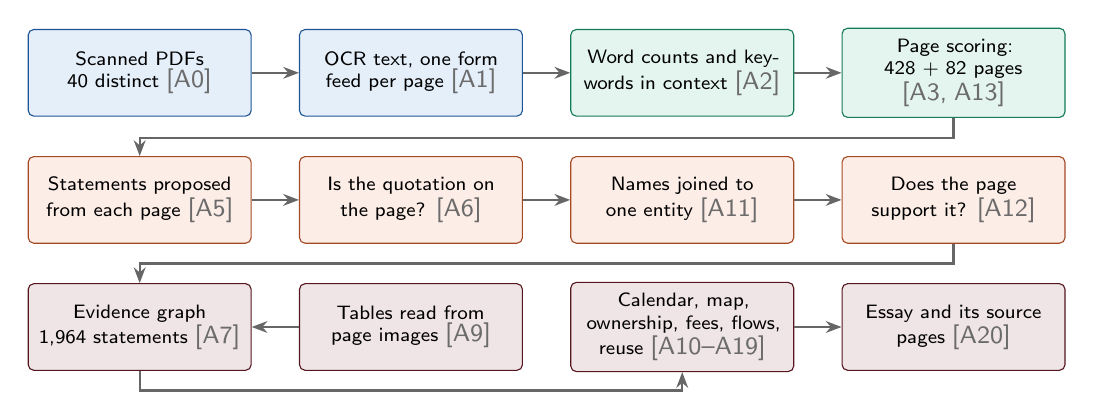
\begin{tikzpicture}[
  node distance=5mm and 6mm,
  box/.style={draw=#1!70!black, fill=#1!12, rounded corners=2pt, align=center, font=\sffamily\scriptsize,
              inner sep=4pt, minimum height=11mm, text width=2.55cm},
  arr/.style={-{Stealth[length=2mm]}, thick, draw=black!60}]
\node[box=cBlue] (a) {Scanned PDFs\\40 distinct \entry{A0}};
\node[box=cBlue, right=of a] (b) {OCR text, one form feed per page \entry{A1}};
\node[box=cGreen, right=of b] (c) {Word counts and keywords in context \entry{A2}};
\node[box=cGreen, right=of c] (d) {Page scoring:\\428 + 82 pages \entry{A3, A13}};
\node[box=cOrange, below=of a] (e) {Statements proposed from each page \entry{A5}};
\node[box=cOrange, right=of e] (f) {Is the quotation on the page? \entry{A6}};
\node[box=cOrange, right=of f] (g) {Names joined to one entity \entry{A11}};
\node[box=cOrange, right=of g] (h) {Does the page support it? \entry{A12}};
\node[box=maroon, below=of e] (i) {Evidence graph\\1,964 statements \entry{A7}};
\node[box=maroon, right=of i] (j) {Tables read from page images \entry{A9}};
\node[box=maroon, right=of j] (k) {Calendar, map, ownership, fees, flows, reuse \entry{A10--A19}};
\node[box=maroon, right=of k] (l) {Essay and its source pages \entry{A20}};
\draw[arr] (a)--(b); \draw[arr] (b)--(c); \draw[arr] (c)--(d);
\draw[arr] (d.south) -- ++(0,-2.5mm) -| (e.north);
\draw[arr] (e)--(f); \draw[arr] (f)--(g); \draw[arr] (g)--(h);
\draw[arr] (h.south) -- ++(0,-2.5mm) -| (i.north);
\draw[arr] (j)--(i); \draw[arr] (i.south) -- ++(0,-2.5mm) -| (k.south); \draw[arr] (k)--(l);
\end{tikzpicture}}
\caption{The pipeline. Blue: preparing the corpus. Green: distant reading. Orange: turning pages into checked statements. Maroon: the evidence base and what we built on it.}\label{fig:pipeline}
\end{figure*}

\subsection{Distant reading: counting words and choosing pages}

We began by counting ten groups of words in every volume: words for flocks, for shepherds, for the herding peoples, for pasture, for season and route, for rights and dues, for the forest and the state, for trade, for debt, and for wage work \entry{A2}. The counts are given per 10,000 words so that long and short volumes can be compared. The script also keeps every match with twenty words on either side, 14,283 of them, so that a pattern in the numbers can always be traced back to real sentences. We kept the names of herding peoples (Gaddi, Gujjar, Kinnaura) apart from the words for shepherds (malundi, pohal, fawal). If we had not, a Gujjar village would have looked like a village of shepherds just because the word ``Gujjar'' is everywhere in it.

The same word groups then helped us decide where to read closely \entry{A3}. There are 3,754 pages in the 1961 volumes, and most of them are about schools, temples and dress. We scored each page and kept it if it had several herding words from several groups, or a word about rights, dues, forest or debt next to a word about flocks or pasture, or a dense run of one kind of word. That left 428 pages, about one in nine. To test the selection, we checked it against the 65 pages we had already cited by hand in Stage~1: it found 56 of them. The nine it missed are easy to explain. Three only say which river a village stands on, four are livestock tables that OCR had turned into number soup, and two mention herding in passing on pages about something else. We entered those by hand or read them from images. For the colonial volumes we used the same scoring, but also required a page to name the hills at least twice, so that plains material dropped out. This kept 82 colonial pages, including all five we had cited \entry{A13}.

\subsection{Close reading at scale: the evidence graph}

Even 510 pages is a lot to read and record by hand in a few weeks, so we used a language model as a first reader, and built the checks around it rather than trusting it \entry{A4--A8}. For each selected page the model proposed short statements in a fixed form: someone, does something, to or with something, with a number, months, place and period where the page gives them, and always with the exact words it relied on. For example: \emph{Forest Department, collects fee from, shepherds, Rs~15 per 100 head per season}, with the quotation from Brahmaur, p.~55.

The rule that holds the whole thing together is simple. \textbf{A statement only enters the graph if a script finds its quotation on the page it cites.} The script allows for small OCR slips, but it insists that every number in the quotation is present. We tested it on purpose with bad inputs. It rejected an invented sentence, a paraphrase, a quotation two pages away, and a quotation with the year changed from 1950 to 1951. One test exposed a real flaw: when we changed ``Rs.~15'' to ``Rs.~25'' in a genuine quotation, the first version of the checker still accepted it, because the rest of the sentence matched so well. We then added the rule about numbers, and after that the altered quotation was rejected.

A quotation can be genuine and the statement still wrong. One proposed statement had Gaddis grazing in Pangi's forests, but its own quotation says they have \emph{no} right to graze there and trespass. So a second, separate pass asked a model to judge every statement against its page as supported, partly supported, or not supported \entry{A12}. Statements judged not supported are left out of all our results.

\begin{table}[!htbp]
\centering\small
\begin{tabularx}{\columnwidth}{@{}>{\raggedright\arraybackslash}Xr@{}}
\toprule
\textbf{Step} & \textbf{Statements}\\
\midrule
Proposed by the model from the 1961 and colonial pages & 1,843\\
Entered by us by hand, from Stage~1 and the evidence packet & 50\\
Read from page images (livestock tables) & 174\\
Rejected because the quotation was not on the page & 44\\
\textbf{Kept in the evidence graph} & \textbf{1,964}\\
\quad judged supported\,/\,partly supported\,/\,not supported & 1,135\,/\,545\,/\,108\\
Graph used for the analyses: places, people and things\,/\,links & 854\,/\,1,856\\
\bottomrule
\end{tabularx}
\caption{From pages to checked statements \entry{A6, A7, A12}.}\label{tab:claims}
\end{table}

The same thing is often called by different names: Brahmaur is also Bharmour and Barmor, and moneylenders appear as sahukars. A model proposed which names belong together, and we went through its proposals. Most were right, but some needed changing \entry{A11}. The best example is the word \emph{ban}. The model wanted to treat it as ordinary pasture, and we first took it for the oak whose leaves are winter fodder. Newell's sentence settles it: ``Each ban in Kangra is claimed by a Gaddi as its warisi (inheritance)'' \pg{Newell}{18}. A \emph{ban} here is a winter grazing run held by inheritance, which is evidence about property in pasture, so we gave it its own entry. In the end, 674 named entities tie the statements together.

\subsection{Methods we chose not to use}

We considered four other methods from the Programming Historian and left them out for reasons that came from the material. \textbf{Topic modelling} would mostly rediscover the chapter headings, because all 24 village surveys follow the same Census template. \textbf{Word embeddings} need far more clean text than our million or so noisy words. \textbf{Sentiment analysis} has nothing reliable to say about the flat prose of census officers. And a \textbf{graph database} would add machinery without adding anything, since a few thousand statements fit easily in plain CSV files.

% ================================================================ 4
\section{What the analyses show}\label{sec:findings}

\subsection{Where the vocabulary falls}

The word counts already sketch the shape of the evidence before any close reading \entry{A2}. Herding words cluster in the high villages: words for flocks run at 27.1 per 10,000 in Brahmaur, about 20 in Maingal and Chitrari and about 18 in Kothi and Kanum, against 6 or 7 in low villages such as Chaunri, Pangna, Shathla and Shakrori. Trade words split the two valleys we compare (Figure~\ref{fig:trade}). The upper Sutlej villages, which traded with Tibet, use them two to four times as often as the Ravi villages, and the Weaving Craft Survey, which reports a shortage of wool and pashm after the Tibet trade stopped, uses them most of all. Words for rights and dues are thickest where the permit system is described: Newell, Devi-Kothi and Brahmaur. Words for the forest and the state are almost absent before 1961 (none at all in 1881 and Rose, 0.04 in 1931), a first hint, from vocabulary alone, that the state forest arrives late in these sources.

\begin{figure}[!htbp]
\centering
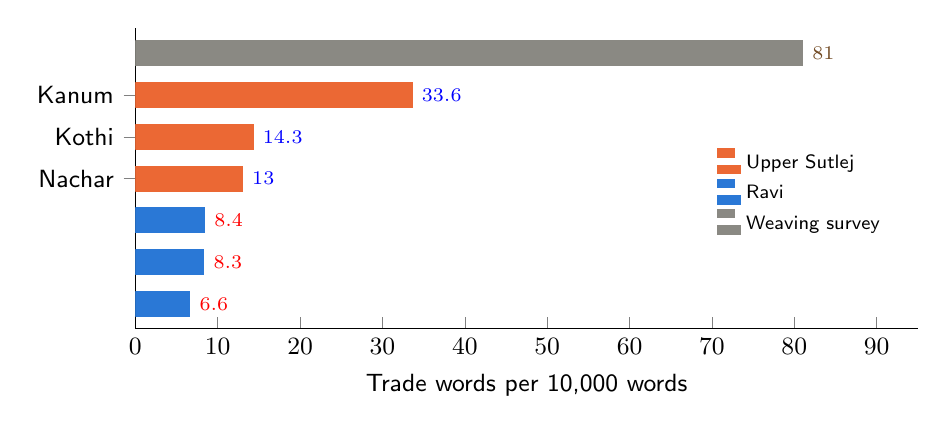
\begin{tikzpicture}
\begin{axis}[
  xbar, width=0.95\columnwidth, height=5.4cm,
  symbolic y coords={Weaving survey,Kanum,Kothi,Nachar,Chitrari,Brahmaur,Maingal},
  ytick=data, y dir=reverse, xmin=0, xmax=95,
  xlabel={\sffamily\small Trade words per 10,000 words},
  nodes near coords, nodes near coords align={horizontal},
  every node near coord/.append style={font=\sffamily\scriptsize},
  bar width=9pt, enlarge y limits=0.1, axis x line*=bottom, axis y line*=left,
  tick label style={font=\sffamily\small},
  legend style={at={(0.97,0.45)},anchor=east,font=\sffamily\scriptsize,draw=none},
  legend cell align=left]
\addplot+[bar shift=0pt,fill=cOrange,draw=cOrange] coordinates {(33.6,Kanum) (14.3,Kothi) (13.0,Nachar)};
\addplot+[bar shift=0pt,fill=cBlue,draw=cBlue] coordinates {(8.4,Chitrari) (8.3,Brahmaur) (6.6,Maingal)};
\addplot+[bar shift=0pt,fill=cGrey,draw=cGrey] coordinates {(81.0,Weaving survey)};
\legend{Upper Sutlej, Ravi, Weaving survey}
\end{axis}
\end{tikzpicture}
\caption{Trade vocabulary separates the Sutlej villages, which faced Tibet, from the Ravi villages, which faced Kangra and the plains \entry{A2}.}\label{fig:trade}
\end{figure}

These counts are a map, not evidence on their own. ``Fees'' also catches school fees, and ``Kangra'' turns up in many contexts. Every claim we actually make rests on statements tied to a page.

\subsection{The mountain year hardly moved}

For the first sub-question we took every statement that names months and drew it as a row on a calendar, grouped by river valley (Figure~\ref{fig:calendar}) \entry{A15}. The Gaddi year is clear. In 1961 the Brahmaur survey says that ``in the beginning of the winter (October and November), the flocks are driven to the low hills of Kangra, Nurpur, Pathankot and Jammu'' \pg{Brahmaur}{55}. Fifty years earlier Rose wrote that ``the yearly exodus to Kangra takes place in October and November, and the return journey in April and May'' \pg{Rose}{297}. In 1881 Barnes, quoted by Ibbetson, said the Gaddis feed their flocks ``half the year (the winter months) in the valleys of Kangra'' \pg{1881}{275}. The Gujjars' move with their buffaloes to the high pastures in summer appears in 1881, 1911 and 1961, and the winter descent of hill people in general appears in 1881, 1919, 1931 and 1961.

\begin{figure}[!p]
\centering
\includegraphics[width=\columnwidth,height=0.93\textheight,keepaspectratio]{calendar/calendar.png}
\caption{The mountain year. Each row is a movement named in the sources with its months, grouped by river valley; the year of the source is in brackets. Blue: winter grounds; orange: summer pastures; green: fairs and markets \entry{A15}.}\label{fig:calendar}
\end{figure}

\begin{finding}
\textbf{Finding.} The months and routes of the herding year are the same in 1881, 1911 and 1961. Because the text-reuse check (Section~\ref{sec:reuse}) shows these accounts do not copy one another, this is the testimony of independent witnesses, not one description repeated.
\end{finding}

The weakness is Kinnaur. The Kanum flocks are away from October to April \pg{Kanum}{85}, but the colonial sources say nothing about the Kinnaur cycle, so the long-term comparison is strong only for the Ravi side.

\subsection{Routes cross from one river system to another}

We located 82 of the 168 places that appear in movement statements, including 16 of the 24 survey villages, using OpenStreetMap and elevation data, and drew 57 routes from 91 statements (Figure~\ref{fig:map}) \entry{A17}. The map shows something the separate surveys do not say outright. Each home village sits in one valley, but the routes cut across ranges. Gaddi flocks leave the Ravi valley, spend the summer in Lahul on the Chenab side and the winter in Kangra on the Beas side. The Kinnaur flocks run down the Sutlej to Bilaspur, Arki and Sirmur, and one line runs east to Tibet. The valley is the unit of settlement and farming; the range between valleys is the unit of herding.

\begin{figure}[!htbp]
\centering
\includegraphics[width=\columnwidth]{maps/routes.png}
\caption{Routes named in the sources: blue to winter grounds, dashed orange to summer pastures, green to fairs and markets. Circles are survey villages, sized by flock \entry{A17}. An interactive version is in \file{analysis/maps/routes.html}.}\label{fig:map}
\end{figure}

\subsection{Who owned the flocks}

The livestock tables are the backbone of the Marxist reading, and the OCR wrecks them, so we read the tables of all 24 village volumes from page images and typed them into a table of 131 rows, one per caste per village \entry{A9}. Castes printed with ``..'' were entered as zero, because who owns nothing matters as much as who owns a lot. The printed totals act as a check: in 15 out of 15 tables that print a total, the rows add up to it. A second reading of the small-print tables at higher resolution changed one figure, Nalag's Rajput goats, from 230 to 239.

\begin{figure}[!htbp]
\centering
\includegraphics[width=\columnwidth]{flocks/ownership_shares.png}
\caption{Share of sheep and goats by caste class in the 19 villages whose surveys print a caste table, ordered by river valley \entry{A10}.}\label{fig:own}
\end{figure}

Across all the caste tables, landholding castes owned 89.3\% of 12,210 sheep and goats, scheduled castes 8.1\% and the Gujjars 1.6\% \entry{A10}. In the big herding villages the share is higher still (Figure~\ref{fig:own}). In Brahmaur, Brahmans and Rajputs held 4,391 of the 4,484 animals, 97.9\%. In Kothi the Rajputs held 2,416 of 2,557; in Kanum the Kanets held 1,744 and the Kolis 83. Even among landholders the flocks were unequal: in Nachar an ordinary family kept 100 to 200 sheep and goats, but ``the Lambardar of the village has about 1,100 strong flock'' \pg{Nachar}{33}. The headman, the state's man in the village, was also its largest owner of animals.

The pattern turns over in the villages of the Yamuna side and the Shimla hills, where flocks are small and mostly goats, and Koli households, a scheduled caste, hold most of them: 91\% in Chaunri, 68\% in Pangna and 60\% in Rajana. At first we thought this was an effect of height. It is not: low Shakrori, Kot and Nalag are more than 95\% landholding too, and the rank correlation between altitude and the landholders' share is $-0.05$, which is to say none at all. The reversal follows the caste make-up of that region, where Kolis are a large part of the farming population.

\begin{finding}
\textbf{Finding.} Wherever herding was big business, the flocks belonged to the landholding castes, at 92 to 99\%. Scheduled caste households owned flocks only where flocks were small, in a region with its own caste structure.
\end{finding}

Who did the herding is a separate question. In Brahmaur families herded their own flocks; hired shepherds (\emph{pohals}) were taken on ``by a very few people in rare cases'' and paid in food, clothes, wool, ``two or four sheep per hundred'' and Rs~2 a month \pg{Brahmaur}{55}. In Kinnaur hired shepherds (\emph{fawals}) mattered more, which is why road wages hurt the owners there, as we show below.

\subsection{Does the mountain predict the flock?}

For the Annales side we asked whether height alone predicts how many animals a household keeps \entry{A18}. We collected the altitude each survey gives for its village (17 of them do, for example ``Brahmaur lies at a height of about 7,000$'$'', p.~11), and the number of households (23 villages), and divided the flock by the households.

\begin{figure}[!htbp]
\centering
\includegraphics[width=\columnwidth]{geography/altitude_flock.png}
\caption{Sheep and goats per household against altitude, coloured by river valley \entry{A18}.}\label{fig:alt}
\end{figure}

The rank correlation is 0.54 over 19 villages (Figure~\ref{fig:alt}). The picture behind that number is sharper than a correlation suggests. In the Ravi, Sutlej and Chenab valleys every village above roughly 2,000\,m keeps between 13 and 45 animals per household (Brahmaur 45.3, Devi-Kothi 22.3, Tandi 21.3, Kothi 20.0, Kanum 16.2, Maingal 13.1), while every village below keeps fewer than six. The one high village with almost no flock, Chaupal at 2,342\,m, lies on the Yamuna side. So height makes large-scale herding possible, but the valley, and the routes that open from it, decide whether it happens. With 19 villages chosen by the Census, not at random, we read this as description, not proof. Low villages still take part in herding in their own way: Bir buys animals from ``Gaddis who wander near about in winter'' \pg{Bir}{43}, and Shakrori from ``the Kinnauras that go by'' \pg{Shakrori}{75}.

\subsection{Permits, fees and the fall in fee-paying flocks}

Newell printed a table of the sheep and goats that paid grazing fees in Brahmaur tahsil each year from 1952--53 to 1961--62 \pg{Newell}{38}. We read it from the page image, which also gave us two years our Stage~1 notes had missed \entry{A16}.

\begin{figure}[!htbp]
\centering
\includegraphics[width=\columnwidth]{fees/fee_flocks.png}
\caption{Fee-paying sheep and goats in Brahmaur tahsil, 1952--53 to 1961--62 \pg{Newell}{38}. The shaded year follows the sheep disease \entry{A16}.}\label{fig:fees}
\end{figure}

Fee-paying animals fell from 73,871 to 54,921, a drop of about a quarter (25.7\%). The shape of the fall matters more than its size (Figure~\ref{fig:fees}). Numbers slipped by only 3\% between 1952 and 1957, dropped by 22\% between 1957 and 1960, and then barely moved. Newell's own note says 1959--60 came after the sheep ``were struck by disease''. But he also says the flocks were ``coming back'' by 1962, while the fee-paying numbers stayed down. Fee-paying numbers count permits, not animals. A disease alone would have been followed by recovery; a cap on permits would not. The series fits the cap better, though it cannot rule the disease out.

The fee itself hardly changed. In 1950 the raja's contractor took about Rs~0.16 per goat and Rs~0.09 per sheep in each grazing district \pg{Newell}{18}; in 1961 the Forest Department took Rs~15 for every hundred head for the summer season, Rs~0.15 an animal \pg{Brahmaur}{55}. What changed was who collected, and how many animals were allowed to graze. ``The Forest Department do not now grant any additional permit for more sheep and goats'' \pg{Brahmaur}{46}. Newell adds what followed: ``these permits are freely bought and sold amongst shepherds so that shepherds have now become closed corporations'' \pg{Newell}{37}.

\begin{finding}
\textbf{Finding.} The price of grazing stayed about the same from the raja to the Forest Department. The number of animals allowed to graze was capped, the permit itself became property, and the herding economy closed in on those who already held permits.
\end{finding}

\subsection{Who took a share of whose product}

To follow the Marxist question through time, we picked out every statement in which one party gives up product, money or labour to another: fees and dues, interest on loans, hired labour, the sale of rights and permits, and the sale of produce. That gave 408 flows, which we sorted by period (Figure~\ref{fig:flows}) \entry{A14}.

\begin{figure*}[!t]
\centering
\includegraphics[width=0.8\textwidth,height=0.78\textheight,keepaspectratio]{surplus/flows.png}
\caption{Who takes a share of whose product, by period. Each band runs from the party who gives (left) to the party who receives (right); numbers count statements in the evidence graph \entry{A14}.}\label{fig:flows}
\end{figure*}

The receiver changes with the period. Under the colonial order the Gaddis paid two masters: whenever they were fined by the Kangra authorities, they used to pay ``a similar penalty into the Chamba treasury'' \pg{1881}{275}. Under the rulers' pastures, up to about 1950, the main receiver was the Raja of Chamba, who owned all grazing rights and auctioned the right to collect fees ``to the highest bidder, who was usually a Gaddi'' \pg{Newell}{18}. So one Gaddi collected from the others on the raja's behalf. After 1948 almost every payment for grazing goes to the Forest Department, from shepherds, graziers, households and permit holders. Running through the whole period is a different kind of taking, through credit and trade, where the moneylender is the largest receiver of all (48 statements among the relations drawn in Figure~\ref{fig:flows}), followed by the shopkeeper and the cooperative society. The Gujjars of Maingal are the clearest case: all of them owned buffaloes, yet ``Gujjar households are cent per cent under debt'', borrowing at 30\% from the same people who bought their milk products \pg{Maingal}{42}.

These counts measure how often the surveys mention a relation, not how much money moved. They tell us who the surveyors saw taking a share, which is a fair guide to the shape of the system but not to its size.

\subsection{Are the sources independent? Text reuse}\label{sec:reuse}

If two sources agree because one copied the other, they are one witness, not two. So we checked every page of every source against every page of the sources written before it, looking for runs of twelve or more words in common, after the method of the Programming Historian's lesson on Passim \entry{A19}. We found 4,698 copied passages. Rose builds on the 1881 census throughout, more than 45,000 words in his three volumes. The 1961 \emph{Special Tables on Scheduled Castes and Scheduled Tribes} reprint more than 27,000 words of Rose and about 8,000 of the 1881 census, so their caste descriptions are colonial text, not 1961 observation. There is even a chain: Barnes's description of the hill Gujjars in 1881 \pg{1881}{267} is copied by Rose \pg{Rose}{346}, and from Rose by the 1961 tables.

\begin{finding}
\textbf{Finding.} The sources we rely on for the herding year are independent. Rose's account of the Gaddi year (p.~297) is not copied from 1881, and Newell copies neither. The persistence of the cycle is therefore real agreement between witnesses.
\end{finding}

% ================================================================ 5
\begin{table*}[!t]
\centering\small
\begin{tabularx}{\textwidth}{@{}>{\raggedright\arraybackslash}p{3.3cm}>{\raggedright\arraybackslash}X>{\raggedright\arraybackslash}X@{}}
\toprule
\textbf{Item} & \textbf{What we had} & \textbf{What it is, and how we found out}\\
\midrule
Kothi livestock table & Three caste rows; Rajput share 94.9\% & A fourth row (Badhi, 11 animals) we had missed; total 2,557, Rajput share 94.5\%. Found on the page image\\
Shakrori goats & 153 & 53 on the page; 153 was an OCR error\\
Four ``unreadable'' tables & Too garbled to use & Readable as images; now entered\\
Brahmaur households & 146 & 99 local households, the ones the livestock table counts\\
Kupha's altitude & 8,550\,ft & That figure belongs to Bhanodi, a halt on the road\\
Koli ownership & An effect of altitude & No link with altitude; a regional caste pattern\\
Newell's 1950 fee rates & Dated before 1948 & They are 1950 rates, after the merger\\
``No additional permit'' & Recorded as issuing permits & It records a refusal of permits\\
\emph{ban} & Pasture, or an oak & A hereditary winter grazing run\\
\bottomrule
\end{tabularx}
\caption{Corrections made by the checks \entry{A4, A9, A11, A12, A18}.}
\end{table*}

\section{Comparing across sources}\label{sec:compare}

Putting the analyses side by side gives a pattern, and it fits the two readings we set out with.

\textbf{What stayed.} Across 1881, 1911, 1931 and 1961 the herding year keeps the same months and the same routes, and the accounts do not copy each other. Height and valley decide where big flocks are kept. This is the slow time of the mountain, and in eighty years we see no sign of it moving.

\textbf{What changed.} Within that fixed year three things moved, and each shows up in a different analysis. The receiver of the herders' surplus moved from the raja and his fee contractor to the Forest Department, with the moneylender and the shopkeeper present throughout. The permit, introduced as a limit on grazing, became something to buy and sell, and the number of fee-paying animals fell by a quarter, mostly in three years. And road work drew away hired labour where the owners depended on it: in Kanum the well-to-do ``found it difficult to engage labourers to attend to their sheep and goats. Men and women now prefer to work on the roads rather than work as `fawals'\,'' \pg{Kanum}{51}.

\textbf{What did not change.} The flocks stayed with the landholding castes. That is the standing fact under every period, and it is why changes in who controlled the pastures mattered so much: they decided how much of the landholders' wealth in animals could be turned into a living, and who took a cut of it.

\textbf{The two valleys.} Comparing the Ravi and the upper Sutlej, as Bloch would, shows geography deciding which outside force reached a valley. The Sutlej faced Tibet. Its villages are full of the vocabulary of trade, and when the border closed after the India--China dispute, ``no more do caravans of mules, flocks of sheep and goats and ladden [\emph{sic}] human beings now wind through the cavernous openings of Shipki-La'' \pg{Kanum}{51}; the Weaving survey records the resulting shortage of wool and pashm \pg{Weaving}{16}. The Ravi faced Kangra and the plains, and the permit system is documented mainly there. The two valleys also started from different kinds of property. On the Ravi the raja owned the grazing and sold the right to collect fees, so pasture was already a revenue farm; in Kanum ``there is no custom to partition the pastural land'' \pg{Kanum}{18}. Our working idea is that the older form shaped the newer one: a revenue farm turned into a market in permits on the Ravi, and common land turned into fenced state land on the Sutlej. We cannot test this fully yet, because the Kinnaur surveys give no grazing dues and the colonial sources do not describe Kinnaur herding.

\textbf{Between the colonial and the 1961 sources.} The colonial layers are good on the cycle and on caste, and silent on grazing dues and pasture ownership in the hills; for those we depend on Newell and the 1961 surveys. The 1961 caste descriptions in the Special Tables turn out to be reprinted colonial ethnography, so we treat them as colonial evidence. The 1931 census was taken at the end of February, when the flocks were away in the low hills, and the report itself says that migration distorts its figures.

\begin{finding}
\textbf{Provisional answer.} Geography fixed the form of the herding year, and it outlasted every change of rule. Property and the state decided who could take part in it and who profited. By 1961 the cycle went on as before, but for fewer, permit-holding owners.
\end{finding}

% ================================================================ 6
\section{Checking our own work}\label{sec:checks}

\subsection{What the checks caught}

Running the pipeline turned up mistakes in our own Stage~1 notes and in our first readings. We list them because they show the computation doing real work, not just decorating conclusions we already had.



The meaning check also checked us: on its first run it judged 11 of our own 41 hand-entered statements unsupported, and we made 17 corrections. The checker has its limits too. Run twice, it gives the same verdict on 77\% of statements, so we treat its verdicts as a filter that removes the worst errors, not as proof. To measure how often it agrees with a person, we drew a random sample of 50 statements, which we are now checking by hand.

\subsection{How we used AI}

Two AI tools did part of this work, and we want a reader to be able to judge it. OpenAI's \emph{gpt-6-luna} proposed the statements from the selected pages, suggested which names belong together, and judged every statement against its page; all of that cost about USD~1.16. Anthropic's Claude wrote the scripts with us, read the livestock tables and Newell's fee table from page images, and helped us draft. The log lists every such step. Nothing an AI produced is used unless its quotation is on the cited page, and the figures read from images are marked as such until one of us has checked them against the scan.

% ================================================================ 7
\section{Where we stand and what is next}\label{sec:next}

The corpus is organised and every page reference can be checked. The evidence graph, the ownership tables, the calendar, the fee series, the flow chart, the route map, the altitude test and the reuse check are built, and every one can be rerun from the repository. A first full draft of the essay exists and is built from these results: every quotation in it is checked by a script against its page, and a companion file reproduces the 64 source pages it cites.

What remains is mostly human checking, and we are doing it in order of how much each item carries the argument:

\begin{enumerate}
\item Check the figures read from page images against the scans, starting with Brahmaur p.~54, Kothi p.~102 and Newell p.~38.
\item Finish the 50-statement sample, so that we can say how often the AI checker agrees with us.
\item Check our caste classes against the 1961 Special Tables, and merge near-duplicate names (``sheep breeder'', ``shepherd'').
\item Find an outside source for the date Shipki La closed, and the Chamba and Kangra settlement reports for grazing rights before 1948, the biggest gap in our sources.
\end{enumerate}

The limits are worth stating plainly. Counts of statements show how often the sources speak of something, not how large it was. Shares are by caste, so they hide inequality inside a caste. The village sample was chosen by the Census, and 19 or 24 villages are too few for statistics beyond description. The colonial sources are silent on Kinnaur, which makes the Sutlej side of our comparison the weaker one.

% ================================================================ appendix
\onecolumn
\appendix
\titleformat{\section}{\Large\sffamily\bfseries\color{maroon}}{Appendix \thesection}{0.7em}{}[{\color{maroon!35}\titlerule}]
\section{The repository}

\url{https://github.com/gamemaker1/history/tree/analysis}

\begin{table}[H]
\centering\small
\begin{tabularx}{\columnwidth}{@{}>{\ttfamily\raggedright\arraybackslash}p{4.2cm}>{\raggedright\arraybackslash}X@{}}
\toprule
\textrm{\textbf{Folder or file}} & \textbf{What it holds}\\
\midrule
sources/ & The scanned sources (Git LFS), with \file{index.md} describing each and giving online copies\\
text/ & OCR text of every source, one form feed per PDF page\\
scripts/ & Every process we ran, one Python script each\\
data/ & What we built by hand or checked: statements, entities, the livestock tables, fees, altitudes, households\\
analysis/ & Everything the scripts produce: the evidence graph and its viewer, calendar, map, ownership, fees, flows, text reuse\\
essay/ & The draft essay and \file{sources.pdf}, the 64 source pages it cites\\
computational-analysis.md & The log of every step, A0 to A20, with commands, results and caveats\\
\bottomrule
\end{tabularx}
\end{table}

The main steps, in order, with their log entries: unpack and check the sources \entry{A0}; count words and choose pages (\file{kwic.py}, \file{candidate_pages.py}) \entry{A2, A3, A13}; propose and check statements (\file{extract_claims.py}, \file{verify_claims.py}, \file{resolve_entities.py}, \file{check_claims.py}) \entry{A5, A6, A11, A12}; read the tables and run the tests (\file{flocks.py}, \file{fees.py}, \file{geography.py}) \entry{A9, A10, A16, A18}; build the graph and its views (\file{build_graph.py}, \file{surplus_graph.py}, \file{calendar_chart.py}, \file{map_routes.py}, \file{text_reuse.py}) \entry{A7, A14, A15, A17, A19}. The full run order, 23 steps, is at the top of the log.

\section{Programming Historian lessons we drew on}

\begin{itemize}
\item \emph{Keywords in Context (Using n-grams) with Python} and \emph{Counting Word Frequencies with Python}: the word counts and keyword-in-context rows \entry{A2}.
\item \emph{Exploring and Analyzing Network Data with Python}: the evidence graph and the flows between parties \entry{A7, A14}.
\item \emph{Geocoding Historical Data}: placing villages, pastures and passes (done in Python, not QGIS) \entry{A17}.
\item \emph{Detecting Text Reuse with Passim}: the method behind our reuse check, written in plain Python \entry{A19}.
\item \emph{Visualizing Data with Bokeh and Pandas} and \emph{Creating Interactive Visualizations with Plotly}: the ideas behind the charts, which we drew with matplotlib.
\end{itemize}


\clearpage
\section{Tools and technologies}

Every tool we used, and what we used it for. All of them are free or open source, except the two AI models, which we paid for or used through a subscription.

{\small
\renewcommand{\arraystretch}{1.22}
\begin{tabularx}{\textwidth}{@{}>{\raggedright\arraybackslash}p{3.6cm}>{\raggedright\arraybackslash}p{2.8cm}>{\raggedright\arraybackslash}X@{}}
\toprule
\textbf{Tool} & \textbf{Kind} & \textbf{What we used it for}\\
\midrule
\multicolumn{3}{@{}l}{\sffamily\bfseries\color{maroon}Preparing the sources}\\
\texttt{pdftotext} (Poppler) & Text extraction & Turning the scanned PDFs that have a text layer into plain text, one page break per PDF page\\
Tesseract & OCR & Reading Rose's \emph{Glossary}, vol.~2, which has no text layer\\
PyMuPDF & Python library & Counting PDF pages to check them against the text, and rendering pages and close-up crops as images to read tables\\
Python \texttt{zipfile}, \texttt{hashlib} & Standard library & Unpacking the source archives and removing duplicate PDFs by checksum\\
\midrule
\multicolumn{3}{@{}l}{\sffamily\bfseries\color{maroon}Analysis}\\
Python 3.12 & Language & Every script in the project, 30 in all\\
\texttt{uv} & Package manager & Installing Python and the libraries inside the project folder\\
Regular expressions (\texttt{re}) & Standard library & Word counts, keywords in context, page scoring, finding altitudes and household totals\\
\texttt{difflib} & Standard library & Fuzzy matching of quotations against OCR text when checking statements\\
pandas & Python library & Tables: ownership by caste, fee series, altitudes, flows, essay evidence\\
NetworkX & Python library & Building the evidence graph and the flows between parties; exporting it as GraphML and Cytoscape JSON\\
Matplotlib & Python library & The charts: calendar, ownership shares, flock size, altitude, fee series, flows\\
\midrule
\multicolumn{3}{@{}l}{\sffamily\bfseries\color{maroon}Maps and places}\\
Folium (Leaflet) & Python library & The interactive route map\\
OpenStreetMap Nominatim & Web service & Finding coordinates for villages, pastures, passes and fairs\\
OpenTopoData (SRTM) & Web service & The height of each located place\\
Wikidata API & Web service & A fallback for places OpenStreetMap could not find\\
OpenTopoMap, OpenStreetMap tiles & Map tiles & The relief and plain backgrounds of the map\\
\texttt{requests} & Python library & Calling the three web services above\\
\midrule
\multicolumn{3}{@{}l}{\sffamily\bfseries\color{maroon}Viewing the graph}\\
Cytoscape.js & JavaScript library & The interactive viewer of the evidence graph and of the flows by period\\
Cytoscape Desktop (optional) & Application & Opening the exported \texttt{.cyjs} files for further layout\\
Google Chrome (headless) & Browser & Taking images of the interactive views, and checking their layout\\
\midrule
\multicolumn{3}{@{}l}{\sffamily\bfseries\color{maroon}AI}\\
OpenAI \emph{gpt-6-luna}, \texttt{openai} SDK & Language model & Proposing statements from pages, joining names to entities, and judging each statement against its page (about USD~1.16 in all)\\
Anthropic Claude, in Claude Code & AI assistant & Writing the scripts with us, reading tables and Newell's fee table from page images, and helping draft the text\\
\midrule
\multicolumn{3}{@{}l}{\sffamily\bfseries\color{maroon}Writing and sharing}\\
\LaTeX{} (pdfLaTeX, TikZ, pgfplots, tcolorbox) & Typesetting & This report, the essay, the pipeline diagram and the trade chart\\
Git, GitHub & Version control & Keeping and sharing the whole project\\
Git LFS & Large-file storage & Storing the scanned sources and other large files (about 600~MB)\\
\bottomrule
\end{tabularx}}

\end{document}
